
%----------------------------------------------------------------------------------------
%   PACKAGES AND OTHER DOCUMENT CONFIGURATIONS
%----------------------------------------------------------------------------------------

% latexmk -pvc -pdf
\documentclass[10pt, a4paper, singlespacing, headsepline]{article}
\usepackage[utf8]{inputenc} % Required for inputting international characters
\usepackage[T1]{fontenc} % Output font encoding for international characters
\usepackage{dsfont}
\usepackage[margin=0.98in]{geometry}
\usepackage{graphicx}
\usepackage[font=scriptsize,labelfont=bf]{caption}
\usepackage{amsmath,amsthm,amsfonts,amssymb}
\usepackage{mathtools}
\usepackage{blindtext}
\usepackage[english]{babel}
\newenvironment{Figure}
    {\par\medskip\noindent\minipage{\linewidth}}
    {\endminipage\par\medskip}

\newcommand\II{\mathbb{I}}
\newcommand\PT{\textit{PT}}
\newcommand\PP{\textit{P}}
\newcommand\TT{\textit{T}}

%----------------------------------------------------------------------------------------
%   TITLE PAGE
%----------------------------------------------------------------------------------------

\begin{document}
\begin{titlepage}
\begin{center}


\vspace{0.5cm}
\textsc{PHS3350 - Physics Project Report} \\
\vspace{2.5cm}

{\Huge Non-Hermicity in quantum mechanics}
\vspace{3cm}

{\LARGE Ana Fabela Hinojosa \footnote{acfab1@student.monash.edu.au}} \\
\vspace{0.4cm}
{\Large Supervisors:\\ Dr. Jesper Levinsen \\ Prof. Meera Parish \\}
\textsc{School of Physics \& Astronomy} \\
\vspace{3cm}

\includegraphics[scale=0.2]{logo.jpg} \\ % University logo
\vspace{3cm}
{\LARGE \today}\\
\vspace{0.5cm}
\end{center}
\end{titlepage}

%----------------------------------------------------------------------------------------
%   QUOTATION PAGE
%----------------------------------------------------------------------------------------

\vspace*{0.2\textheight}

\noindent{``It is not the strongest of the species that survives, 
not the most intelligent that survives. 
It is the one that is the most adaptable to change.''}\bigbreak

\hfill Charles Darwin

\vspace{20cm}

%----------------------------------------------------------------------------------------
%   LIST OF CONTENTS/FIGURES/TABLES PAGES
%----------------------------------------------------------------------------------------

\tableofcontents % Prints the main table of contents

\vspace{20cm}

\listoffigures % Prints the list of figures

\vspace{20cm}

% \listoftables % Prints the list of tables



%----------------------------------------------------------------------------------------
%  CONTENTS
%----------------------------------------------------------------------------------------

\begin{abstract}
\blindtext
\end{abstract}

\section{Introduction}
When my supervisors offered me the possibility of doing my research project on a different kind of quantum theory, I accepted the proposition promptly. 
From early on, my main motivation was to disenfranchise myself from any assumptions about what it meant to do quantum mechanics. I thought that this project could help me in the process of reformulating what I thought I already understood. This did happen, and the more I read about this topic the more I noticed that my picture of quantum theory was not wrong, but it was incomplete. From this realisation my curiosity only grew, as the new information I discovered resembled a set of shinier new tools for my toolbox. I hope that reading this work has the same effect for you.

\subsection{Good ol' quantum mechanics}
In the standard formalism of quantum mechanics operators must satisfy a set of properties which deem them suitable as real observable quantities in nature.
An operator is defined as observable if its eigenvalues are real valued. This means that an observer may use the operator to measure certain qualities of a system and come to a real answer. In addition, it is  necessary that the eigenvalues of the operator are bounded below. Hence, the observer will be able to measure a minimum value out of all the possible real answers. 
The original postulates of quantum mechanics encapsulate these two physical criteria in a mathematical property of operators known as Hermicity (Hermitian operators are also known as self-adjoint operators in mathematics).\\
An operator $\hat{O}$ is Hermitian if it satisfies for any $|f \rangle$ and $|g\rangle$
\begin{equation} \label{eq:1}
\langle f|\widehat{O}|g\rangle = \langle g|\widehat{O}|f \rangle^{*},
\end{equation}  
Where the asterisk operation represents complex conjugation.\\
The equations governing the time evolution of a physical system can be derived from the Hamiltonian of said system\cite{BenderPT}. Nominally, Hermitian Hamiltonians are used to describe systems that are not in contact with their environment. These idealised systems are conventionally called \textit{closed} or \textit{isolated}, these adjectives refer to the defined boundary conditions of the system and how these conditions affect the system dynamics. \textit{Isolated} systems undergo unitary time evolution, Ie. As time passes, the eigenstates' norms are preserved and so the total probability of an eigenstate of the system is conserved. 
\\The reality and boundedness of a Hermitian Hamiltonian's energy spectrum and the unitary time evolution of its eigenstates demonstrate the robustness of Hermicity as a mathematical condition to impose as a postulate in quantum theory.
But with this robustness arise limitations. Because it is not possible to use quantum theory on a system that is in contact with the outside environment.

\subsection{Adopting a new assumption}
The desire to study non-idealised systems using quantum mechanics requires that we reconsider the Hermicity postulate and replace it with one that is less restrictive.
In addition to expanding our analytical tool-box, non-Hermitian quantum mechanics prioritises physical principles rather than mathematical ones by establishing parity-time reflection symmetry (\PT-symmetry) as a more generalisable alternative to Hermicity.
 
\subsection{\PT-symmetric quantum mechanics}
The \PP-operator represents parity (space-reflection), that is, any gain or loss components in a system get interchanged for the opposite component. The \TT-operator represents time-reversal, it has the effect of turning a system with gain into a system with loss (and vice versa)\cite{BenderPT}. In Figure~\ref{fig:AB} on page~\pageref{fig:AB}, I present a toy example of a \PT-symmetric system.
\begin{Figure}
\centering
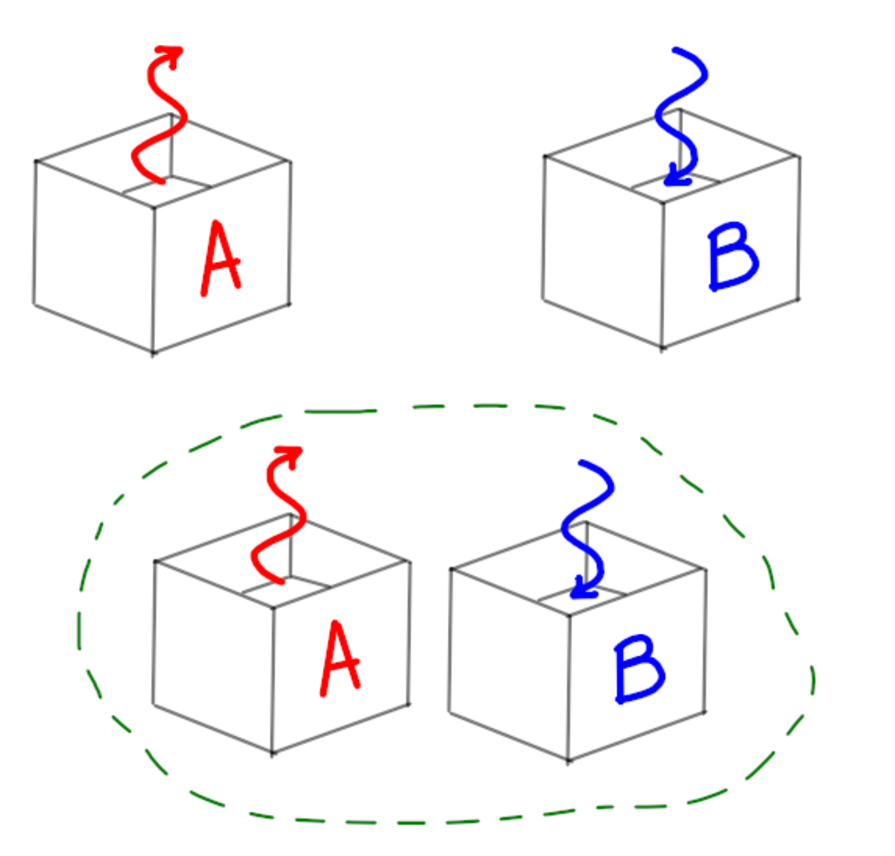
\includegraphics[width=0.4\linewidth]{cartoon1.pdf}
\captionof{figure}{If there are two subsystems, call them A and B, and both subsystems are in contact with the outside environment, where the set-up is that the subsystem A gains energy while subsystem B loses the same amount of energy. Then we can consider the A and B subsystems as time-reversed versions of each other. Taken together as a larger combined system, then the AB system has no net probability flux. Notice that when we exchange A for B there is no change to the composite system, This means that the combined AB system is \PT-symmetric.}
\label{fig:AB}
\end{Figure}
The parity operator ($P$) is defined as a linear, reflection operator with the spatial basis matrix representation:
\begin{equation} \label{eq:2}
P = \begin{bmatrix}
0 & 1 \\ 
1 & 0
\end{bmatrix},
\end{equation}
Notice that $P^2 = 1$. In addition, the \PP-operator is equal to its inverse $P = P^{-1}$.\\
The time-reversal symmetry operator ($T$) is defined as antilinear in order to preserve the Heisenberg commutation relation $[\hat{x}, \hat{p}] = i\hbar$\cite{BenderPT} and thus be consistent with the time dependent Schrödinger equation\cite{Jones-Smith}.
The antilinearity of $T$ is defined as 
\begin{equation} \label{eq:3}
T \psi T^{-1}= L \psi^{*},
\end{equation}  
$T$ acts as complex conjugation of a state $\psi$ followed by a linear operator $L$ (which may or not be Hermitian) acting on the state. There are two kinds of time-reversal: Even and odd, that is $T^2 = 1$ and $T^2 = -1$ respectively. These two kinds of time-reversal symmetry apply to different particles. In the case of Bosons (integer spin) only even \TT-symmetry applies. while odd \TT-symmetry applies exclusively to Fermions (half-integer spin)\cite{Jones-Smith}.
The scope of this work will focus exclusively in the case of even \TT-symmetry. With this simplification we can work with a basis such that 
\begin{equation} \label{eq:4}
T \psi T^{-1} = \psi^{*}.
\end{equation}
By focusing on even \TT-symmetry we can consider $T$ as a reflection operator as we do with $P$. The $T$ doesn't have a spatial basis matrix representation.
Since parity and time-reversal operation are independent of each other, then the $P$ and $T$ operators commute\cite{BenderPT}.\\
In Figure~\ref{fig:AB} on page~\pageref{fig:AB} we considered a very simple case of a composite \PT-symmetric system, where the composition involved combining a subsystem A with its time-reversed version B.
Let us imagine that A can be described with the simple $1 \times 1 $ Hamiltonian $H_{A} = [a+ib]$ where $a, b \in \mathds{R}$, since we established that B is simply the time-reversed version of A then B's Hamiltonian is $H_{B} = T (H_{A}) T^{-1} = [a-ib]$.\\
We can write the Hamiltonian of the composite AB system as the $2 \times 2$ Hamiltonian matrix
\begin{equation} \label{eq:5}
H_{\mathrm{AB}} = \begin{bmatrix}
a+ib & 0 \\ 
0 & a-ib
\end{bmatrix}.
\end{equation}
$H_{AB}$ is not Hermitian, but we can prove that it is \PT-symmetric:
\begin{equation} \label{eq:6}
PT(H_{\mathrm{AB}})T^{-1}P^{-1} = \begin{bmatrix}
0 & 1 \\ 
1 & 0
\end{bmatrix}
T
\begin{bmatrix}
a+ib & 0 \\ 
0 & a-ib
\end{bmatrix}
T^{-1}
\begin{bmatrix}
0 & 1 \\ 
1 & 0
\end{bmatrix},
\end{equation}

\begin{equation} \label{eq:7}
\therefore PT(H_{\mathrm{AB}})T^{-1}P^{-1} = \begin{bmatrix}
0 & 1 \\ 
1 & 0
\end{bmatrix}
\begin{bmatrix}
a-ib & 0 \\ 
0 & a+ib
\end{bmatrix}
\begin{bmatrix}
0 & 1 \\ 
1 & 0
\end{bmatrix}
\end{equation}

\begin{equation} \label{eq:8}
\therefore PT(H_{\mathrm{AB}})T^{-1}P^{-1} = 
\begin{bmatrix}
a+ib & 0 \\ 
0 & a-ib
\end{bmatrix}
\end{equation}

\begin{equation} \label{eq:9}
\therefore PT(H_{\mathrm{AB}})T^{-1}P^{-1} = H_{\mathrm{AB}}
\end{equation}
The system described by equation (\ref{eq:5}) is not in dynamic equilibrium since as time evolves, the norm of the states of subsystem A decay and those of B grow. If we implement a coupling parameter $g$ between our subsystems, then the states of A and B will be coupled and so we can write the composite coupled-state Hamiltonian as 
\begin{equation} \label{eq:10}
H_{\mathrm{coupled}} = 
\begin{bmatrix}
a+ib & g \\ 
g & a-ib
\end{bmatrix}
\end{equation}
Notice that \PT-symmetry is preserved in equation (\ref{eq:10}). The coupling strength $g$ determines the reality of the eigenvalue spectrum of $H_{\mathrm{coupled}}$.
To see this, we solve the eigenvalue problem
\begin{equation} \label{eq:11}
\mathrm{det}(H_{\mathrm{coupled}}-IE) = a^2 +b^2 + E^2 -g^2 -2aE
\end{equation} \label{eq:11}
where $I$ is the identity matrix and $E$ are the eigenvalues we want to find. Notice that the second order polynomial in equation (\ref{eq:11}) is real. The roots of this polynomial are 
\begin{equation} \label{eq:12}
E_{\pm} = a \pm \sqrt{g^2 - b^2},
\end{equation}
from this we can derive 3 scenarios, the first is the case when $g^2 < b^2$. In this case we have complex-valued eigenvalues, and so the weak coupling scenario yields a system that is not in dynamic equilibrium, because the coupled states continue to decay or grow. Alternatively, if $g^2 > b^2$ then this corresponds to strongly coupled states that do not decay nor grow, and so we have a real valued energy spectrum. These two coupling scenarios correspond to the cases of broken and unbroken \PT-symmetry respectively. Finally the last case is when $g = \pm b$. This is the degenerate case. In non-Hermitian system degeneracy is expressed by real eigenvalues merging into complex conjugate pairs as $|g| \rightarrow b$. In my discussion I will explain on how the merging of eigenvalues has important experimental consequences.

\subsection{Nerd-Sniped}
\begin{Figure}
\centering
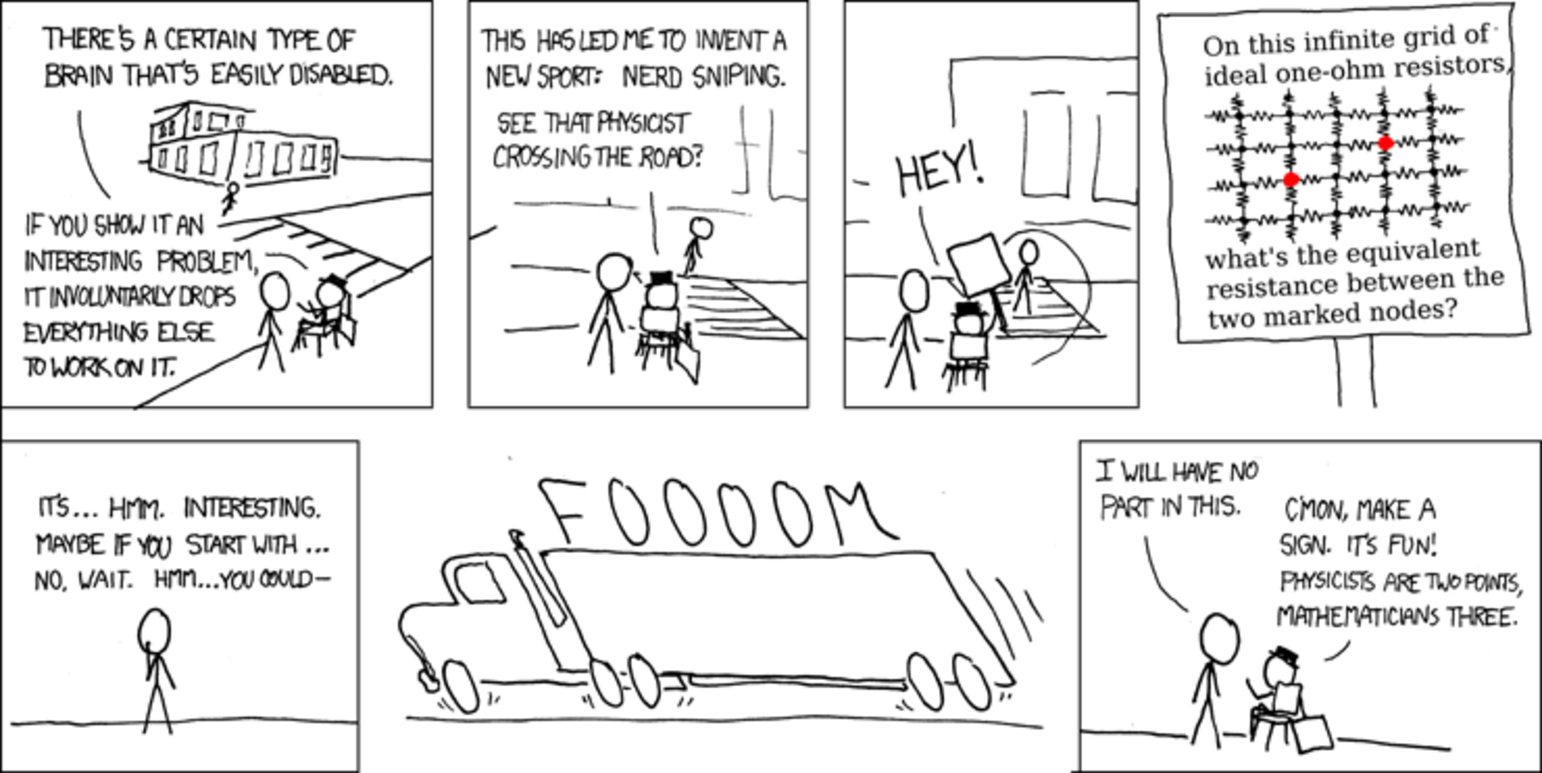
\includegraphics[width=0.6\linewidth]{nerd_sniping.pdf}
\captionof{figure}{The relevant XKCD comic -Nerd Sniping- https://xkcd.com/356/. Illustrates what happened to me during my project. }
\end{Figure}
I must be honest, I had a couple of ideas for my project but I only achieved one of them. Early on in the semester while I was reading ``Making sense of non-Hermitian Hamiltonians'' by Carl Bender I encountered a really interesting figure.

\begin{Figure}
\centering
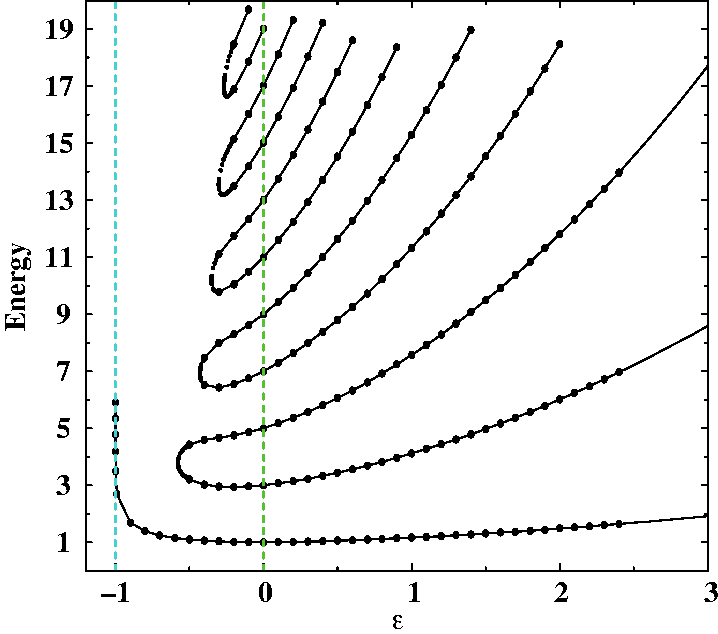
\includegraphics[width=0.5\linewidth]{figure_1_Bender.pdf}
\captionof{figure}{This is Figure 1. in reference \cite{Bender}. It exemplifies the behaviour of the eigenvalue spectra of the general parametric family of non-Hermitian Hamiltonians $\hat{H} = \hat{p}^2 + \hat{x}^2 (i \hat{x})^{\epsilon}$ as a function of the real parameter $\epsilon$. All the eigenvalues visible in this figure are real valued. The \PT-symmetry breaks at the $\epsilon = 0$, which corresponds to the Hamiltonian for the classic one dimensional harmonic oscillator. When $\epsilon \geq 0$ the spectra are real, positive and discrete. Energy levels increase with increasing $\epsilon$. In the region  corresponding to $-1 \leq \epsilon \leq 0$ there is a finite number of real positive eigenvalues and an infinite number of complex-conjugate pairs of eigenvalues (not depicted). The number of real eigenvalues decreases as $\epsilon$ decreases from $0$ to $-1$, for $\epsilon$ that are more negative than the value $\epsilon = -0.57793$ the only remaining real eigenvalue corresponds to the ground-state energy. At the value $\epsilon = -1$ the spectrum is null, as all the eigenvalues diverge to infinity.}
\label{fig:Benders}
\end{Figure}

My investigations of non-Hermitian Hamiltonians were pivoted by trying to understand what was going on in the figure above. My approach to understanding was based on trying to replicate the figure itself as it portrays a very clear visualisation of \PT-symmetry breaking (occurring at $\epsilon = 0$) and its effect on the energy spectrum of non-Hermitian \PT-symmetric Hamiltonians $\hat{H} = \hat{p}^2 + \hat{x}^2 (i \hat{x})^{\epsilon}$. It can be seen in this figure that the reality and boundedness from below of the eigenvalues is maintained as the perturbation parameter $\epsilon$ is varied.\\

For my investigation of this figure, I had to solve the time independent eigenvalue problems associated with a $\hat{H} = \hat{p}^2 + \hat{x}^2 (i \hat{x})^{\epsilon}$. For this I used two different mathematical techniques, since the reality of the spectrum for \PT-symmetric Hamiltonian systems is characterized by the commutation relation of the Hamiltonian in question and the \PT-operator. The meaning of broken and unbroken \PT-symmetry is defined as a conditional statement: \textit{If the Hamiltonian and the \PT-operator share all eigenstates, then the symmetry is unbroken, but if not all the eigenstates are simultaneously shared between the Hamiltonian and the \PT-operator then the symmetry is broken}\cite{BenderPT}\cite{Bender}. In other words, only if the \PT-symmetric Hamiltonian shares eigenstates with the \PT-operator, then the corresponding eigenvalues to those shared eigenstates are real-valued.

Replicating this figure took most of my time during the semester, and so I was unable to develop my other investigations further. Nevertheless, for the sake of completeness, I will describe in section 2 what my other project idea was.

\section{My aborted simulation}
\subsection{Methods}
According to ``Non-Hermitian quantum mechanics'' by Nimrod Moiseyev. A book that I was given by my supervisors early on in the semester. The numerical propagation of wave packets is much more simple when taken within the framework of the non-Hermitian formalism of quantum mechanics rather than in the standard (Hermitian) formalism\cite{Moiseyev}. The main idea behind this method is to include a reflection-free complex absorbing potential (RF-CAP) in the Hamiltonian describing the wave packet's time evolution. This added potential term allows the description of outward flowing states without any un-physical reflection effects from the boundary of the simulation region.\\
I was very eager to verify this technique on a simulation of a wave packet propagating in space using Python. First, I constructed wave function to be propagated. Since I required analytically verifiable derivatives, I figured that the easiest wave function choice was a Gaussian wave packet with initial condition 
\begin{equation} \label{eq:13}
\psi(x, 0) = e^{-(x^2/2\sigma^2)}e^{ik_{0}x},
\end{equation}
where $x \in \mathds{R}$, $\sigma = 1$ and $k_{0} = 10$. In order to implement the time evolution of my wave function, I used the 1D Schrödinger equation
 \begin{equation} \label{eq:14}
\frac{d}{dt}\psi(x, t) = \frac{-i}{\hbar} \left [ \frac{-\hbar^2}{2m} \frac{d^2}{dx^2} + V(x, t)\right ] \psi(x, t),
\end{equation}
To numerically calculate the second order spatial derivative I used the Fourier transform property \mbox{$\mathcal{F}\{f'(x)\} = ik\mathcal{F}\{f(x)\}$}, then my equation became
\begin{equation} \label{eq:15}
f(x, t, \psi) =  \frac{-i}{\hbar} \left [ \frac{-\hbar^2}{2m} \mathcal{F}^{-1}\{-k^2\mathcal{F}\{\psi(x, t)\}\} + V(x, t)\psi(x, t)\right ],
\end{equation}
I was originally unsure of what the potential $V(x,t)$ should look like since the whole point of this exercise is the inclusion of a reflection-free complex absorbing potential (RF-CAP) in the Hamiltonian. The RF-CAP should attain non-zero values only in the boundary region in the coordinate space where the physical potential $V(x,t)$ vanishes\cite{Moiseyev}. Eventually, I opted for implementing a square well potential as $V(x,t)$ in the Schrödinger equation to give rise to the non-physical interference that should be expected at the boundary of the coordinate space given the non continuous boundary conditions the problem requires.
I defined the square well potential V(x, t) as an array over an x array ranging from $0$ to $10$. The square potential was defined as zero everywhere except at the boundaries. The boundaries' height was determined by trial and error based on the kinetic energy of the wave packet. I settled the barrier to be a thousand times larger than the initial value for the wave vector squared, \mbox{ie. $V(0, t) = V(10, t) = 1000k_0^2$}.\\\\
Implementing the time evolution required by the simulation I used the fourth-order Runge-Kutta method on equation (\ref{eq:15}) $f(x, t, \psi)$. The algorithm is defined as
\begin{equation} \label{eq:16}
\begin{split}
&k_1 = f(x, t, \psi),\\
&k_2 = f(x, t + \frac{\Delta t}{2}, \psi + \frac{1}{2}k_1),\\
&k_3 = f(x, t + \frac{\Delta t}{2}, \psi + \frac{1}{2}k_2),\\
&k_4 = f(x, t + \Delta t, \psi + k_3),\\
&\psi_{n + 1} = \psi_{n} + \frac{1}{6}(k_1 + 2k_2 + 2k_3 + k_4) + O(\Delta t^5).\\
\end{split}
\end{equation}
where $\Delta t = 0.0001$ is the evolution time step, I chose this value to be small enough to be able to resolve motion of the Nyquist mode within the spatial step 
$\Delta x = \frac{x_{\mathrm{max}} - x_{\mathrm{min}}}{1024} = \frac{10}{1024}$.
This numerical formula in equation (\ref{eq:16}) propagates a solution over a time interval by combining the information obtained by solve a differential equation using four Euler-style steps (each involving one evaluation of the differential equation with slightly different parameters), and then using the information obtained to match a Taylor series expansion up to fourth order, by combining the evaluations if the differential equation in this way we eliminate the error terms order by order, with the error remaining being very small\cite{N_R}.

\subsection{Results}

\begin{Figure}
\centering
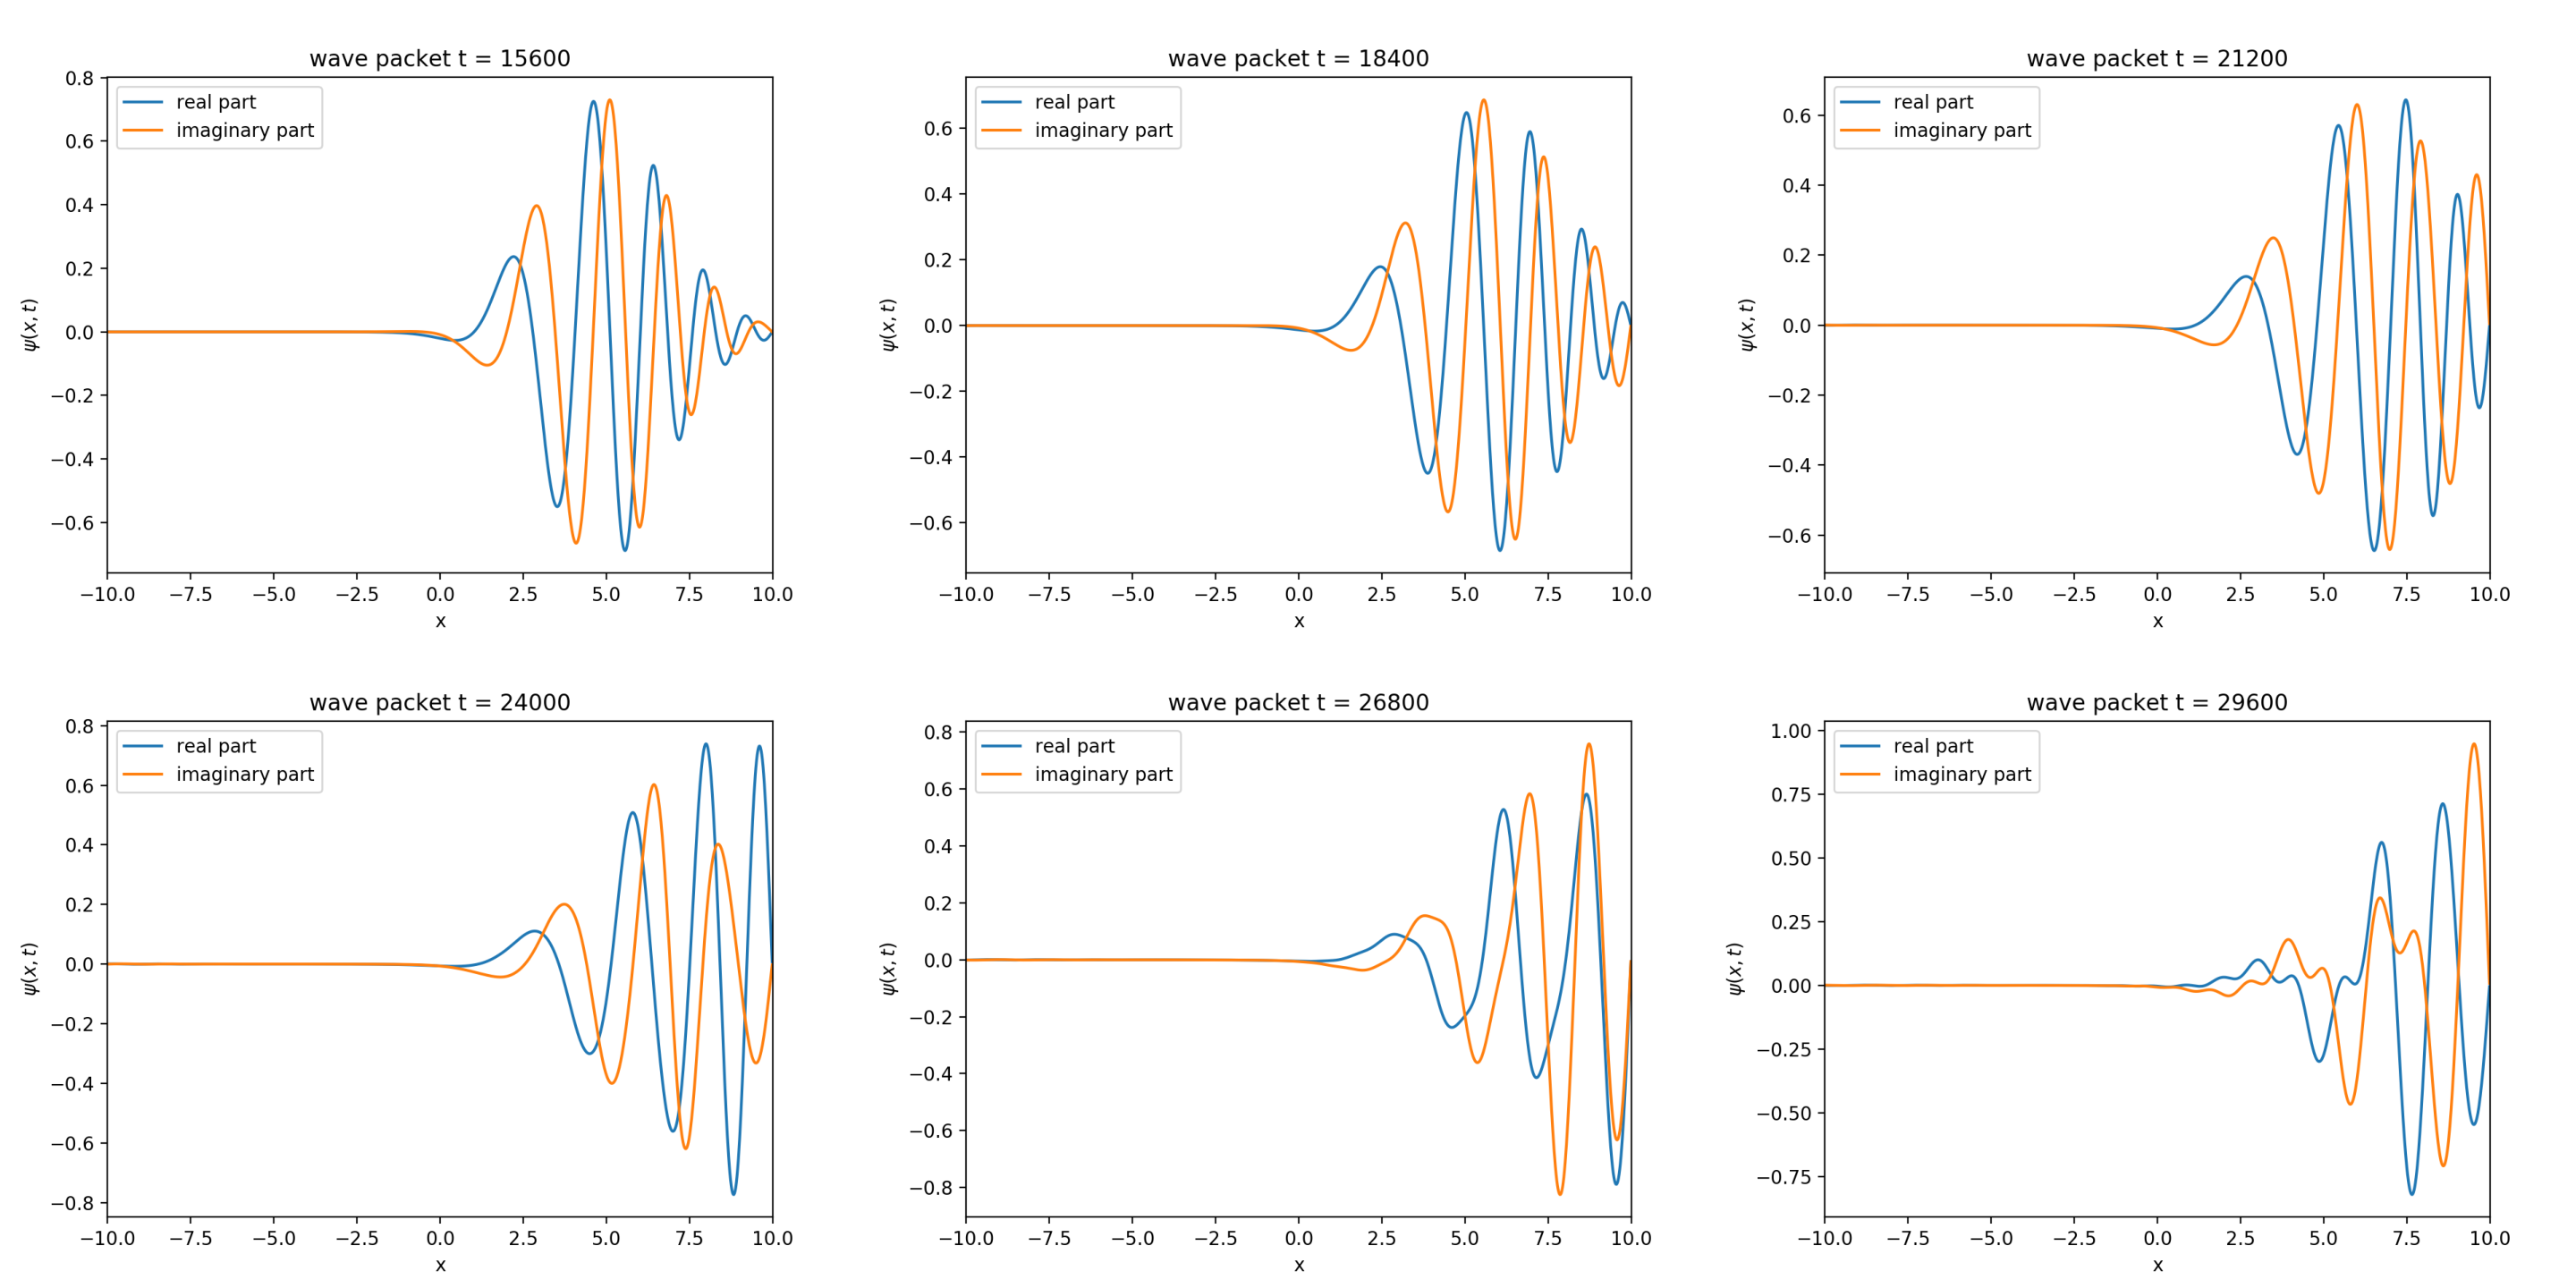
\includegraphics[width=\linewidth]{propagating_wave_with_reflection.pdf}
\captionof{figure}{These are 6 frames of my simulation of a right propagating Gaussian wave packet in space as a function of time.The horizontal axes of every frame correspond to the spatial coordinate x (dimensionless) and the vertical axes of every frame correspond to the real and imaginary parts of the Gaussian wave packet. The earliest time frame is the top left panel, corresponding to wave packet at time t =  15600 as can be seen in that plot's title. An ``undesirable" reflection of the real part of the wave packet at the boundary is visible specially in the last 3 frames from left to right, corresponding to times t = 24000, t = 26800 and t = 29600 as can be seen in the plots' titles from left to right respectively.}
\end{Figure}
Understanding the implementation of the potential characteristic to this non-Hermitian technique simulation required a lot of reading and I ambitiously decided to leave this project unfinished in the meantime and continue with it after I successfully replicated Figure 1. in Bender. A project which I naively expected to finish quickly.

\section{Reproducing Bender's figure}

The defining principle behind Figure~\ref{fig:Benders} on page~\pageref{fig:Benders} is that we can think of the family of non-Hermitian \PT-symmetric Hamiltonians in equation (\ref{eq:17}) as complex deformations of the 1D harmonic oscillator (which is Hermitian and \PT-symmetric).
\begin{equation}\label{eq:17}
\hat{H} = \hat{p}^2 + \hat{x}^2 (i \hat{x})^{\epsilon},
\end{equation}
where $\epsilon$ is a real parameter. The introduction of the real parameter $\epsilon$ acts in such a way that as $\epsilon$ increases from $0$, the Hamiltonian is no longer Hermitian but its \PT-symmetry is preserved. This occurs because the quantity $(i\hat{x})$ is \PT-invariant\cite{BenderPT}\cite{Bender}.\\ 
To formulate the eigenvalue problems for both methods used to find all the eigenvalues of equation (\ref{eq:17}), I split the problem into the expected parametric regions (as per Bender's descriptions) corresponding to \textit{unbroken} \PT-symmetry ($\epsilon \geq 0$) and \textit{broken} \PT-symmetry ($\epsilon < 0$).\\
When $\epsilon \geq 0$ the spectra are real, positive and discrete. Energy levels increase with increasing $\epsilon$.
To solve the Schrödinger eigenvalue problem I write the Schrödinger equation in coordinate space.\\ The relevant operators in this space are
\begin{align} \label{eq:18}
\hat{x}& \rightarrow x,  &\hat{p}\rightarrow -i \frac{d}{dx},
\end{align}
where we want to treat the variable x as complex, which does not modify the commutation relation $[\hat{x}, \hat{p}] = i\hbar$. Then the eigenvalue problem takes the form
\begin{equation}\label{eq:19}
-\psi'' + x^2 (i x)^{\epsilon} \psi = E \psi.
\end{equation}
Equation (\ref{eq:19}) cannot be solved exactly using analytic methods for $\epsilon \neq 0$, therefore my approach is numerical. From reference \cite{Bender} I learned that the WKB phase integral approximation can be used to find very a accurate approximation to the real eigenvalues visible in the \textit{unbroken} \PT-symmetry region ($\epsilon \geq 0$) visible in Figure~\ref{fig:Benders} on page~\pageref{fig:Benders}. 

\subsection{Methods}

\subsubsection{WKB approximation}
To solve equation (\ref{eq:19}) I had to find out which were the boundary conditions for the problem. I learned from several sources that the boundary conditions depend on the deformation parameter $\epsilon$ \cite{BenderPT}\cite{Bender}\cite{Bender2017}. Since the eigenvalue problem can be conceptualised as a harmonic oscillator that has been deformed into the complex x-plane, finding the solutions requires that I integrate equation (\ref{eq:19}) along a contour in the complex x-plane and that the solution be equal to zero at both ends of this contour\cite{BenderPT}. According to Bender, the integration contour should be located within two angular sectors in the complex x-plane as $|x| \rightarrow \infty$. These sectors are called \textit{Stokes wedges}\cite{BenderPT}\cite{Bender}, in general these wedges are centred about the origin in the complex x-plane and are defined as 
\begin{align} \label{eq:20}
&-\frac{1}{4} \pi  < \mathrm{arg}x < \frac{1}{4}\pi& &\mathrm{and}& &\frac{3}{4} \pi  < \mathrm{arg}x < \frac{5}{4}\pi& 
\end{align}
the eigenfunctions of the problem vanish exponentially at both ends of the integration contour.\
Determining the locations of the \textit{Stokes wedges} is in general not necessary to solve the differential equation exactly\cite{BenderPT}. For the purpose of my eigenvalue problem, it is only required to understand the asymptotic behaviour of the solutions for large $|x|$ values.\\
I assumed that for an ODE of the form of equation (\ref{eq:19}), ie. \mbox{$\psi'' V(x)^{\epsilon} \psi = E \psi$}, the behaviour of $(E - V(x)) \rightarrow \infty$ as $|x| \rightarrow \infty$ in the complex x-plane. The next assumption I made was that the solution should be of the form
\begin{equation} \label{eq:21}
\mbox{$\psi \approx \mathrm{exp}[\pm  \int^{x}dx \sqrt{E - V(x)}]$},
\end{equation}
this is called the \textit{geometrical-optics approximation}\cite{BenderPT}.\\ 
The location of \textit{Stokes wedges} in the complex plane, and hence the defined boundary conditions for my problem are determined by imposing that \mbox{$\psi(x) \rightarrow 0$ as $|x| \rightarrow \infty$} similarly to the case where $\epsilon = 0$ ie. The classical harmonic oscillator case,where the solutions are known to be square integrable for real x-values.\\
Since I am assuming that my solutions will be wave functions moving in space, I am interested in learning how much phase is gained by traversing the integration contour in the complex x-plane. The end points of the integration contour are the turning points (the roots of the equation $E = x^2(ix)^{\epsilon}$) that \textit{analytically continue} off the real axis as $\epsilon$ increases from $0$\cite{BenderPT}\cite{Bender}. Independently of the number of possible roots of $E = x^2(ix)^{\epsilon}$, for the purpose of my technique I only need the following turning points to be the limits of integration
\begin{align} \label{eq:22}
x_{-}& = 
E^{\frac{1}{\epsilon + 2}}
e^{i\pi(\frac{3}{2} - \frac{1}{\epsilon + 2})}
&\mathrm{and}&
&x_{+} = E^{\frac{1}{\epsilon + 2}} e^{-i\pi(\frac{1}{2} - \frac{1}{\epsilon + 2})}.
\end{align}
The explicit formula I used in my numerical calculation of the eigenvalues is the the leading order WKB phase integral quantization condition 
\begin{equation} \label{eq:23}
\left (n +\frac{1}{2}\right )\pi = \int^{x_{+}}_{x_{-}}dx \sqrt{E - x^2(ix)^{\epsilon}},
\end{equation}
as per Bender's instructions in ``Making sense of non-Hermitian Hamiltonians''. the left hand side of equation (\ref{eq:23}) is the quantization condition on the accumulated phase for the WKB integral that defines the energy.\\



% \subsubsection{Matrix diagonalisation}


% \subsection{Results}

% \subsubsection{The region of unbroken \PT-symmetry}


% I calculated how much phase is gained by traversing a contour in the complex plane from one of the roots of the equation $E = x^2(ix)^\epsilon$ to the other.


% % \begin{equation}
% % (n+ \frac{1}{2})\pi = \int_{x_-}^{x^+} dx \sqrt{E - x^2(ix)^\epsilon}.
% % \end{equation}

% % I reproduced the results reported in Bender's paper by using the WKB approximation.

% % I had to devise a way to write the complex integral using Python and this required a change of variables that shifted my integration limits and domain from the complex plane to the real line. I did this taking advantage of the symmetry of the setup by subtracting as an offset the imaginary part multiplied by $i$ of one of the integration limits from both of the limits and from the integrand. 

% % Even though I encountered some difficulties, in the end my implementation of the WKB method returned results that were in agreement with those reported in Bender's paper. Demonstrating that the WKB methodology gives a very accurate approximation to the exact eigenvalues reported by Bender (obtained by using Runge-Kutta) for the case of the unbroken symmetry sector of the spectrum in figure 1. (ie. when $\epsilon > 0$).


% \subsubsection{The region of broken \PT-symmetry}


% % \begin{equation}
% % (n+ \frac{1}{2})\pi = \int_{x_-}^{x^+} dx \sqrt{E - x^2(ix)^\epsilon}.
% % \end{equation}

% % I reproduced the results reported in Bender's paper by using the WKB approximation.

% % \begin{Figure}
% %  \centering
% %  \includegraphics[width=\linewidth]{WKB_agreement.png}
% %  \captionof{figure}{From left to right the image is zoomed. Here I demonstrate that my WKB results (blue plot) are in agreement with the values reported in Bender's work. Bender's results were obtained by the Runge-Kutta method (orange plot) and by the WKB approximation (green plot). All the energies presented in this plot were obtained using 
% % $\epsilon = 1$ and $n \in [0,9]$.}
% % \end{Figure}

% % \begin{Figure}
% %  \centering
% %  \includegraphics[width=0.5\linewidth]{unbroken_symmetry_spectrum.png}
% %  \captionof{figure}{Unbroken \PT-symmetry region of the energy spectrum for the parametric family of Hamiltonians
% %  \mbox{$\hat{H} = \hat{p}^2 + \hat{x}^2 (i \hat{x})^\epsilon$} obtained using the WKB approximation.}
% % \end{Figure}




% \section{Discussion}

% \subsection{Stokes wedges and boundary conditions}


% \subsection{\PT-symmetry breaking}



% The known Gaussian-behaviour of the solutions of the undeformed harmonic oscillator, is preserved as the integration contour is deformed into the complex x-plane....
% As $\epsilon$ becomes negative... read page 79 onward

% there is no continuous path joining the limits of integration when $\epsilon \leq 0$ therefore the WKB approximation cannot be used in the region corresponding to Broken \PT-symmetry.




% \subsection{Exceptional points}
% % Square-root singularities are often called exceptional points. In general, eigenvalues cross (that is, they become degenerate) at exceptional points, the order of the degeneracy depends on the number of coalescent eigenvalues at that point. An exceptional point also marks the boundary between broken and unbroken \PT- symmetric phases\cite{BenderPT}.

% %The conventional picture of quantum mechanics is that the energy levels are discrete and quantized functions of the real coupling constant $g$, However from the more general complex-variable perspective in which the coupling constant is complex, we can see that the energy levels of a hamiltonian are in fact continuous functions of the complex coupling constant $g$\cite{BenderPT}. 

% % From the behaviour of the Eigenvalues of the Hamiltonian we can see that quantization has a topological interpretation. Note that there are two eigenvalues because there are two sheets in the Riemann surface, following a closed continuous path in the complex-g plane that does not wind around an exceptional point, the energy levels follow closed paths in the complex energy plane, however if the closed path encircles an exceptional point, the energy levels exchange their identities because they are analytic continuations of one another. This phenomenon is called level crossing, and it has been observed experimentally in Gao et al.

% % When we extend the parameters (the coupling constants) of a Hamiltonian into the complex domain, we find that the energy eigenvalues are all branches of a multivvalued function , they are analytical continuations of one another and can be continuously deformed into one another by varying the parameters. Energy levels are in a one to one correspondence with the sheets of a Riemann surface. From the narrow perspective of real variables this topological interpretation is invisible.








% \section{Conclusion}


% \section{Acknowledgements}


% % \section{Appendix}
% %----------------------------------------------------------------------------------------
% %   ABBREVIATIONS
% %----------------------------------------------------------------------------------------

% % \begin{abbreviations}{ll} % Include a list of abbreviations (a table of two columns)

% % \textbf{LAH} & \textbf{L}ist \textbf{A}bbreviations \textbf{H}ere\\
% % \textbf{WSF} & \textbf{W}hat (it) \textbf{S}tands \textbf{F}or\\

% % \end{abbreviations}

\bibliography{mybib}
\bibliographystyle{unsrt}
\end{document}